\documentclass{sig-alternate}
%\documentclass{sig_alternate}
\usepackage[utf8]{inputenc}
\usepackage{graphicx}
\usepackage{algorithm}
\usepackage{algorithmicx}
\usepackage{algpseudocode}
\usepackage{amsmath}


\begin{document}
	\title{An efficient implementation of Online Arithmetic}
	
	\numberofauthors{2}
	
	\author{
		\alignauthor
		Yiren Zhao\\
		\affaddr{Imperial College London}\\
		\affaddr{London, UK, SW7 2AZ}\\
		\email {yiren.zhao13@imperial.ac.uk}
		\alignauthor
		George A. Constantinides\\
		\affaddr{Imperial College London}\\
		\affaddr{London, UK, SW7 2AZ}\\
		\email {g.constantinides@imperial.ac.uk}
	}
	\date{September 2015}
	
	\maketitle
	
	\begin{abstract}
		The unique feature of an Online operator is that it generates results starting from the most significant digit (MSD). This allows numerical precision to be controlled at run-time. In this paper, we report on an optimized FPGA architecture for Online operators to perform efficient serial addition, multiplication and division. We compare these operators with conventional fixed-point arithmetic, over multiple precisions. Using our proposed FPGA implementation, we demonstrate a novel feature in our implementation of providing numerical results to an arbitrary precision at run-time without any increase in circuit area. 
	\end{abstract}
	
	
	\section{Introduction}
    Traditional fixed-point arithmetic operators, both parallel and serial, require precision to be defined at design time. These operations fall into two categories; some, such as multiplication, proceed from the lest significant digit(LSD) to the most significant digit(MSD), while others, such as division, computes from the MSD to LSD. As a result, fixed-point arithmetic performs number-by-number computations: it only takes a new number once finishes calculation of all digits within the previous number. Parallel fixed-point operators have a smaller latency compare with serial operators; nevertheless, they consume increasing hardware resources while precision increases. 
	
	Online arithmetic unifies all arithmetic operations in a MSD-first fashion. Parallel Online arithmetic requires precision to be confirmed at design time, however, serial Online arithmetic allows successive computations to generate answers digit-by-digit. 
	It ensures an output digit of a number to be immediately fed into following operations without finishing generation of all digits in that number. 
	This enables production of results with arbitrary precision: we could connect Online operators and generate results to an unlimited precision at run-time. 
	Because of its capability of generating results with arbitrary precision, serial Online arithmetic could achieve early decision making and thus early termination of calculations. 
	For instance, to compare a fractional number with $0$, we could achieve an early decision once its MSD is generated to be greater or smaller than $0$. In contrast, in order to make a valid comparison, fixed-point arithmetic has to calculate this fractional number in all precisions from LSD to MSD.
	
	Serial Online operators contain the features mentioned above, besides, it only uses a fixed amount of circuitry. Therefore, we discovered a novel way to provide arbitrary precision generation with a non-growing piece of hardware and our implementation could track to any precision at run-time without knowing what precision is needed before running.   
	
	In later sections, an introduction to Online arithmetic and correlated algorithms are given, and optimized hardware architectures are discussed.	
	We make following contributions in this paper:
	\begin{itemize}
		\item Novel implementation of Online arithmetic to generate numerical results to an arbitrary precision with fixed circuitry.
		\item Optimization on hardware architectures of serial Online multiplier and divider.
		\item Evaluation of serial Online operators based on Newton's method.   
	\end{itemize}
	\section{Background}
	Online arithmetic has been broadly exploited in the fields of control and signal processing \cite{online_control}\cite{online_signal_processing}. Recently, it has also proved its usage in over-clocking computations \cite{Kan_overclocking}. Online arithmetic has some unique features due to the algorithms that it relies on. Firstly, the digits are always taken from the MSD (left to right) and the resulting output always contains an initial delay, which is called the Online delay and denoted by $\delta$ \cite{digital_arithmetic_book}. Second feature is that Online arithmetic employs redundant number representation system. To unify the use of representations, in this paper, all implementations only involve digits in signed representation (SD) in a redundant digit set of \{-1,0,1\}, which we denote \{$\bar{1}$,0,1\} for the ease of presenting. 
	
	For each given n-digit operand, we could apply a left-to-right indexing system for its serial computation to the jth iteration, meanwhile, we take considerations of $\delta$ to make this indexing of inputs ($x[j]$ and $y[j]$) and output ($z[j]$) consistent. Since we apply radix-2 system in this paper,  the value of $r$ is equivalent to 2 in equation(1)\cite{digital_arithmetic_book}.
	\begin{equation}
	 x[j]=\sum_{i=1}^{j+\delta}x_{i}r^{-i},y[j]=\sum_{i=1}^{j+\delta}y_{i}r^{-i},z[j]=\sum_{i=1}^{j}z_{i}r^{-i},
	\end{equation}
	
	For each digit $x_{i}$ of this n-digit operand, that has a value within the set of  \{$\bar{1}$,0,1\},  it is represented using 2  bits in SD representation. We denote $x_i^+$ and $x_i^-$ to be the two bits of representing a single digit $x_{i}$, and a subtraction between $x_i^+$ and $x_i^-$ could produce the value of the represented digit(2). This redundancy within the SD representation gives opportunities to represent a conventional number in multiple ways, for instance, the binary number $0.0101$ could be represented as $0.1\bar{1}01$ or $0.011\bar{1}$ and also other alternatives. 
	\begin{equation}
		x_{i}= SUB (x_i^+,x_i^-);
	\end{equation}
	
	\section{Online operators}
	
	\subsection{Addition}
	
	Addition is an important arithmetic operation and it is used for constructing multiplier and divider as well. The serial Online addition makes use of full adders and D flip flops to add two redundant digits, therefore, it contains 2 cycles of online delay ($\delta_{add} = 2$) \cite{arithmetic_overview}. Similarly, if we duplicate this serial adder n times and take out the flip flops, we obtained a n-digit parallel adder without any online dealys \cite{Kan_parallel_operators}. 
	Typically, in the implementation of serial Online multiplication and division, a 4-digit parallel Online adder is applied to avoid Online addition delay and also partially unrolling the serial operation loop, this unrolling would be fully analyzed in later sections. Nevertheless, a serial Online adder is employed in this paper to achieve addition serially in order to solve the Newton's method to the 2nd iteration in later sections.   
	\vspace{-10pt}
	\begin{figure} [ht]
		\centering
		\includegraphics[height=2in,width=3in]{Adder}
		\caption{Online Adder}
	\end{figure}
	\vspace{-5pt}
	\subsection{Multiplication and its Optimization}
	\subsubsection{Multiplication}
	Multiplication requires recursive operations, within which two intermediate residues are produced, respectively named $v[j]$ and $w[j]$. 
	Meanwhile, for each iteration, a corresponding product digit, $p_{j+1}$, is produced by a selection function. This selection process is implemented as a multiplexer in hardware (Algorithm 1) and named $SELM()$ for this multiplication\cite{online_mul}. Typically, such Online multiplication has an online delay, and in this case, $\delta_{mul}=3$ \cite{online_mul}. 
	
	The $SELM()$ function could also be viewed as a sampling process: threshold values categorize upper digits of $v[j]$ and then produce $p_{j+1}$. The threshold values are based on the radix number $r$ and delay value $\delta_{mul}$\cite{online_mul}. Typically, in the radix-2 multiplication implemented in this paper, this sampling process follows equation(3), therefore, we need to track 5 MSDs of the residue, including two integer digits and three fractional digits to reach the precision of the thresholds in equation(3). In hardware, we feed these five MSDs into a multiplexer and select appropriate $p_{j+1}$ with respect to the threshold values \cite{online_mul}. 
	
	
	To multiply one digit with a series of digits, for instance, performing $x[j]y_{j+1}$, is a relatively simple process in hardware. Since $y_{j+1}$ takes value from the digit set $\{\bar{1},0,1\}$, this translates to hardware as choosing whether to negate, zero or maintain the value of each digit in $x[j]$.   
		  
	\begin{algorithm}
		\begin{algorithmic}[1]
			\State {Initialize:\newline $x[-\delta_{mul}]=y[-\delta_{mul}] =v[-\delta_{mul}] =w[-\delta_{mul}] = 0$}\newline
	
			\For {j=$-\delta_{mul}$, $-\delta_{mul}$+1, ... ,n-1}
				\State $v[j] = 2w[j] + (x[j]y_{j+1}+y[j+1]x_{j})2^{-3};$
				\State $p_{j+1} = SELM(v[j]);$
				\State $w[j+1] = v[j] - p_{j+1};$
			\EndFor
		\end{algorithmic}
		\caption{Online Multiplication}
		\label{alg:algorithm1}
	\end{algorithm}	
	\begin{equation}
		SELM (v[j]) = \begin{cases}
		1 &\text{if $v[j] \geq 1/2$}\\
		0 &\text{if $-1/2 \leq v[j] \leq1/4$}\\
		-1 &\text{if $v[j]<-3/4$ }
		\end{cases} 
	\end{equation}
	
	\subsubsection{Optimization of Multiplication}
	Apart from these standard hardware implementations, some optimizations are done to speed up the process and also decrease the usage of hardware resources. The optimizations mainly focus on the addition and subtraction in Algorithm1.
	\begin{figure} [ht]
		\centering
		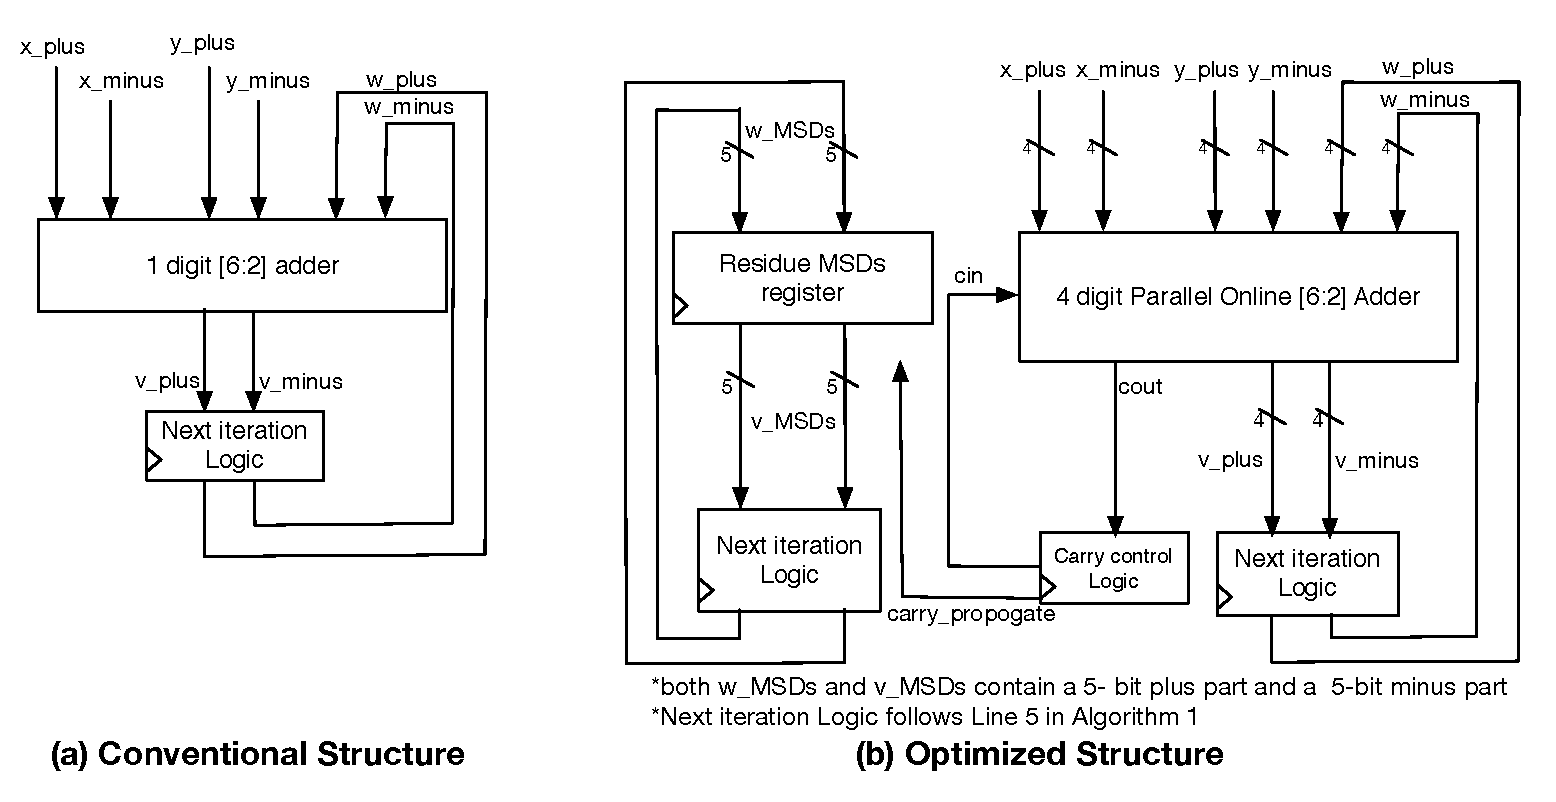
\includegraphics[height=2.7in,width=3.6in]{dividing_upper_block}
		\caption{Online Multiplier}
	\end{figure}
	\vspace{-10pt}
	
	Firstly, standard digit serial multiplication employs serial addition and subtraction, nevertheless, we propose a partially unrolled 4-digit parallel Online adder to speed up the adding process, which theoretically improves the speed by 4x. Secondly, due to the shifting caused by $2^{-3}$, 5 MSDs of residue $v[j]$, including 2 integer digits and 3 fractional digits, remain unchanged unless a carry is propagated from its LSDs. We managed to hold the 5 MSDs in two separated 5-bit registers and thus they only change values if carry logic detects a valid propagation (Figure 2(b)). In an unoptimized design, these 5 MSDs of residue value join addition of every single iteration. Our implementation avoids these unnecessary additions, and thus saves hardware resources by 40 LUTs on Altera Cyclone IV series FPGA.     
	
	\subsection{Division and its optimizations}
	\subsubsection{Division}
	In division, we denote $x$ and $d$ to represent the numerator and divisor respectively. The algorithm of Online division is similar to multiplication at first glance, however, there are inherent differences in terms of selection process and recurrence (Algorithm 2).
	
	
	 The selection process requires more precise threshold vales down to $1/8$ (equation 4), so that six MSDs (two integer digits and four fractional digits) are required to join this SELD multiplexer to produce one digit quotient $q_{j+1}$.  

	          
  
  \begin{algorithm}
		  	\begin{algorithmic}[1]
		  		\State {Initialize:\newline $n[-\delta_{div}]=d[-\delta_{div}] =v[-\delta_{div}] =w[-\delta_{div}] = 0$}\newline
		  		
		  		\For {j=$-\delta_{div}$, $-\delta_{div}$+1, ... ,n-1}
		  		\State $v[j] = 2w[j] + (x_{j+1}-q[j]d_{j+1})2^{-4};$
		  		\State $q_{j+1} = SELD(v[j]);$
		  		\State $w[j+1] = v[j] - q_{j+1}d[j+1];$
		  		\EndFor
		  	\end{algorithmic}
		  	\caption{Online Division}
		  	\label{alg:algorithm2}
  \end{algorithm}	
  \begin{equation}
  SELD (v[j]) = \begin{cases}
  1 &\text{if $v[j] \geq 1/4$}\\
  0 &\text{if $-1/4 \leq v[j] \leq1/8$}\\
  -1 &\text{if $v[j]<-1/2$ }
  \end{cases} 
  \end{equation}
  
  \subsubsection{Optimization of Division}
  	Although Online divider's hardware implementation contains unrolling of the adder and separation of residue's MSDs. The division process contains one more optimization which is related to its algorithm's recurrence. Conventionally, in a single iteration, residue $v[j]$ has to be produced first to provide a $q_{j+1}$ that is later used to produce $w[j+1]$ (Figure 3a). Practically, we find that productions of $v[j]$ and $w[j+1]$ are both time-consuming procedures and heavily increase the latency of our hardware design. Moreover, both procedures cost compatible cycles to finish, denote $m$ to represent this cycle number, and conventional method requires $2m$ cycles to finish computation of one single iteration. Additionally, $m$ grows linearly with the number of iterations $j$, because the size of residue $v[j]$ and $w[j]$ would expand as number of iterations increases.    
   	
  	\begin{figure} [ht]
  		\centering
  		\includegraphics[height=3in,width=3.6in]{flowchart}
  		\caption{Flow chart of Online divider's working mechanism}
  	\end{figure}  	
  To overcome this latency problem, we choose to introduce a prediction mechanism based on previous quotient value. This prediction adds parallelism into hardware design: computing both $v[j]$ and $w[j+1]$ in $m$ cycles. We predict $q_{j}$ might be the same value as before, and therefore uses $q_{j-1}$ to compute the $w_{j+1}$. To the worst case, if prediction fails, the system would branch back to recompute the value of $w_{j+1}$ with a corrected quotient value. Notice that the process of determine whether $q_{j}$ is equal to $q_{j-1}$ is purely logic circuitry, therefore, does not cost any extra clock cycles. 

  Following this optimized design, if the prediction succeeds, we would save our computation cycles by half, decreasing from $2m$ cycles to $m$ cycles. In contrast, if the prediction fails, our method would take up to $2m$ cycles, which is the same as the conventional method. The success rate of this prediction depends on the values of inputing operands, in this case, the numerator digits and divisor digits respectively. The only extra hardware cost in this case is the logic that determines whether the 2-bit quotient digit is the same as before or not. This only costs 1 LE in Cyclone IV FPGA, however, brings us a possibility of speeding up a single iteration by 2x. 
  
  \section{Evaluation}   
  To further study the advantages of Online arithmetic in arbitrary precision control, we choose to chain the operators together in an iterative algorithm. We recall the Newton's Method of finding $\sqrt{3}$ and unroll this iterative algorithm to its second iteration.
    
  	\begin{algorithm}
  		\begin{algorithmic}[1]
  			\State Initialize: $x_{0}=2, f(x)=x^{2}-3, f'(x)=2x$	
  			\For {j=$0$,$1$}
  			\State $x_{j+1}=x_{j}-\frac{f(x_j)}{f'(x_j)};$
  			\EndFor
  		\end{algorithmic}
  		\caption{Newton's Method with two iterations}
  		\label{alg:algorithm3}
  	\end{algorithm}
%To fully visualize the algorithm in terms of data path, we could apply a tree structure of operators to represent one %iteration in Newton's method (Figure 4).  
%\vspace{-8pt}
%\begin{figure} [ht]
%	\centering
%	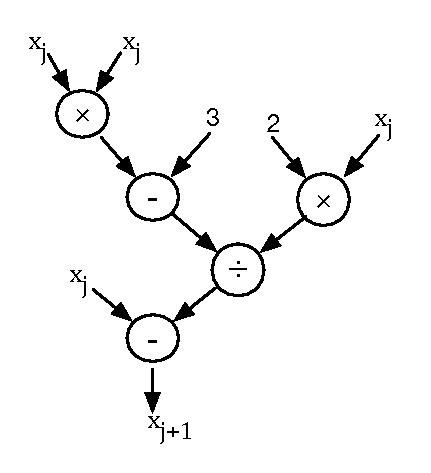
\includegraphics[scale=0.5]{parsing_tree}
%	\caption{Data path of one iteration in Newton's method}
%\end{figure}
%\vspace{-8pt}
For Online arithmetic, the initial Online delay, $\delta$, in this case, would be additive and increase linearly with the number of operators. For example, for one iteration of Newton's method, the total Online dealy of $x_{j+1}$ would be $\delta_{total}$, which is a summation of two $\delta_{mul}$, two $\delta_{minus}$ and one $\delta_{div}$. In other words, the first MSD of $x_{j+1}$ would come out $\delta_{total}$ cycles later after we feed in the fist MSD of $x_{j}$.\newpage
\begin{figure} [ht]
	\centering
	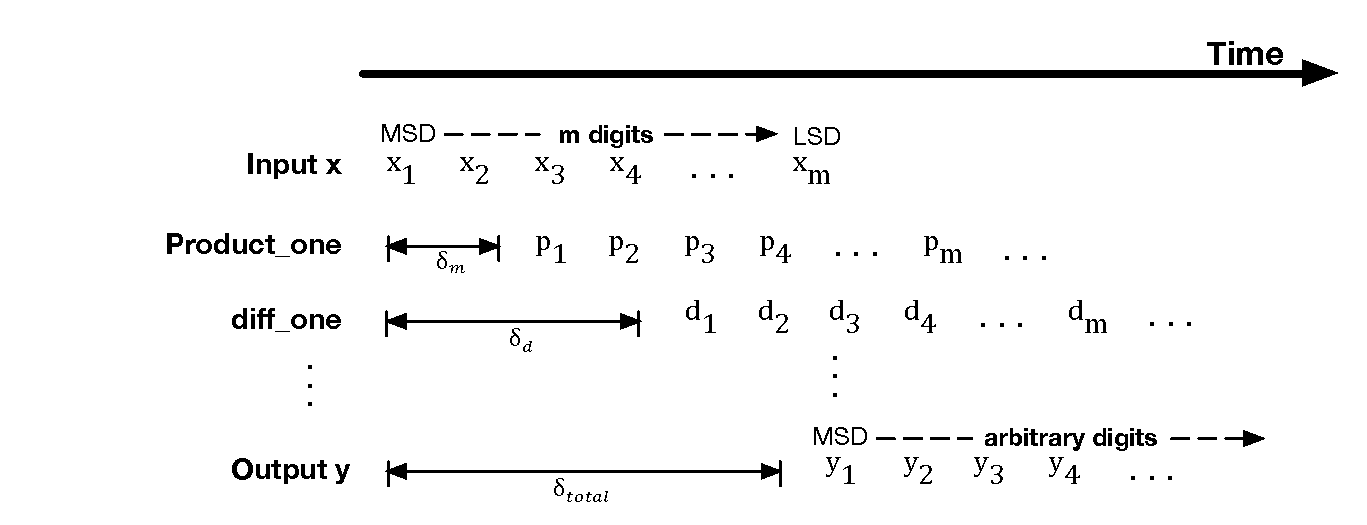
\includegraphics[width=3.3in,height=1.6in]{newton_timing}
	\caption{Timing of Newton's method}
\end{figure}
\vspace{-12pt}

Despite this small Online delay, the unique feature of Online arithmetic makes it able to produce all results, including intermediate results,in a MSD first fashion (Figure 4). 

In this experiment, we compare our novel hardware implementation with conventional fixed-point arithmetic.
Altera Cyclone IV FPGA is selected as the hardware platform for our design and we collect results after Place and Route in Quartus II.   
Fixed-point operators are implemented by IP cores provided by Altera. We choose to use fixed-point operators to perform parallel computations, assuming the precision of these computations are already specified. The correctness of hardware results are verified with the co-simulation in Matlab. Notice we generated results with precision of 8 digits, 16 digits, 32 digits, 64 digits and 128 digits for Online arithmetic. 

\begin{figure} [ht]
	\centering
	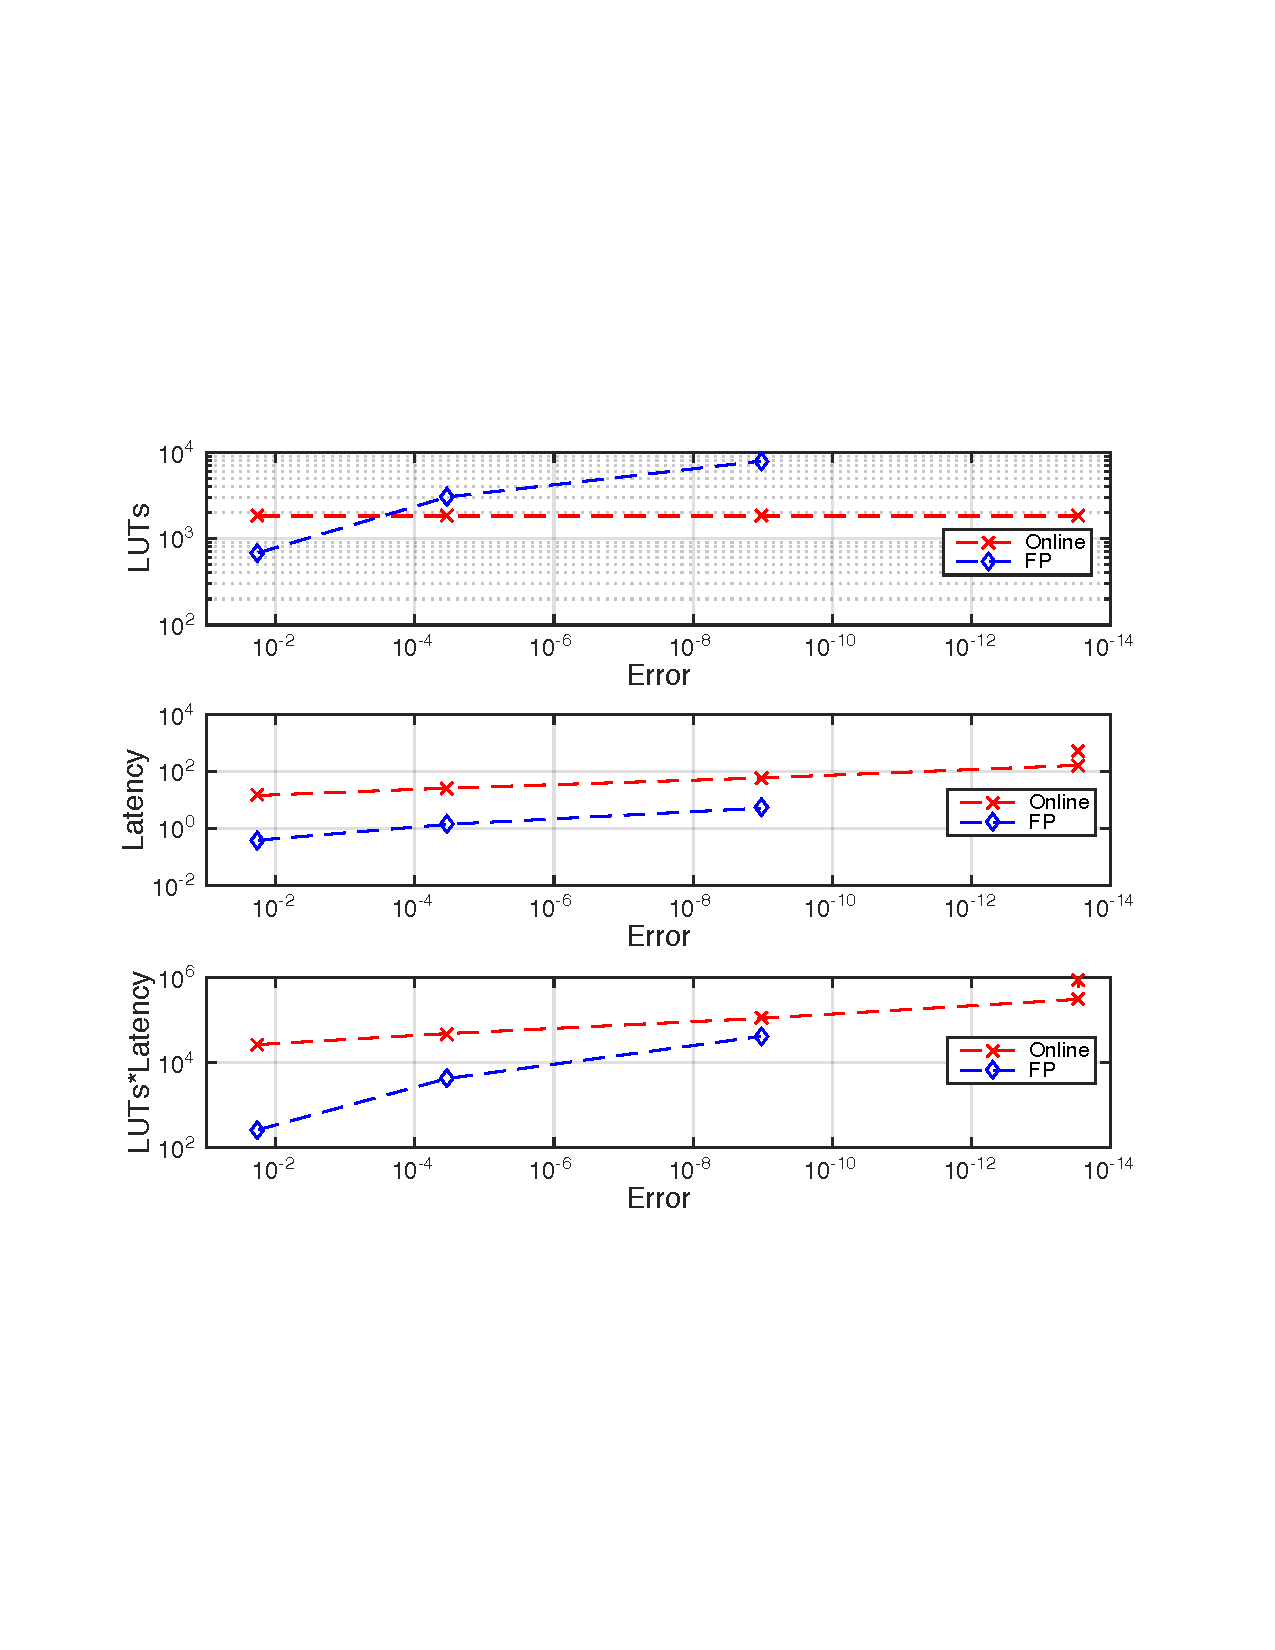
\includegraphics[width= 3.3in, height = 3.8in]{figure101}
	\caption{Comparison between Online and FP arithmetics in terms of latency and number of LUTs used}
\end{figure}
\vspace{-10pt}

As illustrated in the graphs, our implementation's precision grows as time increases. The error value stops decreasing for the Online arithmetic after reaching 64-bit precision (around $10^{-13}$), because it reaches the precision limitation of Matlab. On the other hand, the error decrease of fixed-point operators stops early at 32 bits precision (around $10^{-9}$), because Altera IP cores only performs maximally 32-bit integer division and multiplication in fixed-point arithmetic\cite{altera}, which restricts this error decrease.    

The hardware usage remains (number of LUTs) constant for Online arithmetic, but increasing heavily with fixed-point arithmetic.The initial latency of Online arithmetic is higher due to the accumulation of Online delays, however, grows less dramatically comparing with fixed-point. With the product of LUTs and latency on y axis, two arithmetics become compatible when error is around $10^{-9}$ (32 digit precision).According to the trend observed from these figures, our implementation could have less hardware usage than parallel fixed-point operators when error is less than $10^{-4}$ (around 16 digits precision). Moreover,our piece of hardware could provide results with arbitrary precision at run-time.

\section{Conclusion}
Ultimately, we exploited a novel method of computing numerical answers with arbitrary precision. This method's hardware usage does not grow with increasing precision and is capable of producing arbitrary precision at runt-ime. By comparing our proposed method with parallel fixed-point operators, our implementation with Online arithmetic is predicted to have a better performance and constant hardware usage when required precision is high (above 64 digits precision). Moreover, our method has an ability of computing answers with any precisions if run-time is large enough, due to the uniqueness of Online arithmetic.  


	\bibliographystyle{acm} 
	\bibliography{citation101}
	
\end{document}